% So the image fits the page
\documentclass[class=minimal,border=0pt]{standalone}
% Include tikz
\usepackage{tikz}
\usetikzlibrary{shapes, patterns}
% Define some lovely colours
\definecolor{light-gray}{gray}{0.95}

\begin{document}

\begin{center}
    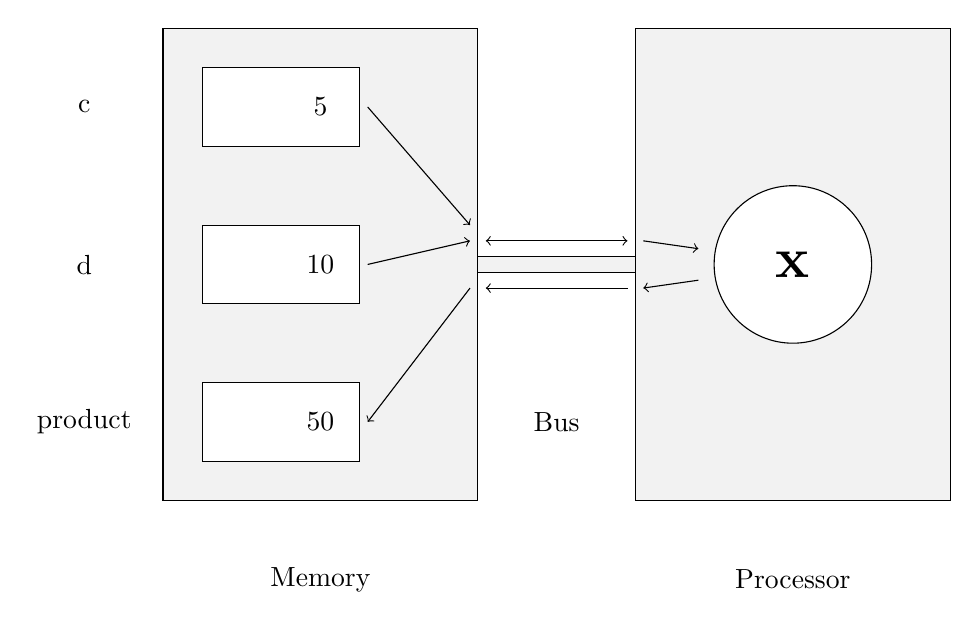
\begin{tikzpicture}
        % Memory box
        \draw [fill=light-gray] (-5,  3) rectangle (-1, -3);
        % Memory label
        \node at (-3, -4) {Memory};
        % 5 box
        \draw [fill=white] (-4.5,  2.5) rectangle (-2.5, 1.5);
        \node at (-3, 2) {5};
        % 5 to bus arrow
        \draw [->] (-2.4, 2) -- (-1.1, 0.5);
        % c label
        \node at (-6, 2) {c};
        % 10 box
        \draw [fill=white] (-4.5,  0.5) rectangle (-2.5, -0.5);
        \node at (-3, 0) {10};
        % 10 to bus arrow
        \draw [->] (-2.4, 0) -- (-1.1, 0.3);
        % d label
        \node at (-6, 0) {d};
        % 50 box
        \draw [fill=white] (-4.5,  -1.5) rectangle (-2.5, -2.5);
        \node at (-3, -2) {50};
        % Bus to 50 arrow
        \draw [->] (-1.1, -0.3) -- (-2.4, -2);
        % product label
        \node at (-6, -2) {product};
        % Bus rectangle
        \draw [fill=light-gray] (-1, 0.1) rectangle (1, -0.1);
        % Bottom bus arrow
        \draw [<-] (-0.9, -0.3) -- (0.9, -0.3);
        % Top bus arrow
        \draw [<->] (-0.9, 0.3) -- (0.9, 0.3);
        % Bus label
        \node at (0, -2) {Bus};
        % Processor box
                \draw [fill=light-gray] (1,  3) rectangle (5, -3);
                % Bus to processor
        \draw [->] (1.1, 0.3) -- (1.8, 0.2);
        % Processor to bus
        \draw [<-] (1.1, -0.3) -- (1.8, -0.2);
                % Processor label
        \node at (3, -4) {Processor};
        % Multiplication circle
        \draw [fill=white] (3, 0) circle [radius=1];
        \node at (3, 0) {\huge \bf x};
    \end{tikzpicture}
\end{center}

\end{document}
